\documentclass[letter, 10pt]{article}
\usepackage[spanish]{varioref}
\usepackage[activeacute,spanish]{babel}
\usepackage{amsfonts}
\usepackage{amsmath}
\usepackage{graphicx}
\usepackage[noend]{algpseudocode}
\usepackage{dsfont}
\usepackage{algorithm}
\usepackage{graphicx}
%\usepackage[ruled,vlined]{algorithm2e}
\usepackage{listings}
\usepackage{url}
\usepackage[top=3cm,bottom=3cm,left=3.5cm,right=3.5cm,footskip=1.5cm,headheight=1.5cm,headsep=.5cm,textheight=3cm]{geometry}

\usepackage[utf8]{inputenc}
\usepackage[T1]{fontenc}


\begin{document}
\title{Inteligencia Artificial \\ \begin{Large}Estado del Arte: Aircraf Landing Scheduling Problem (ALSP)\end{Large}}
\author{David Medel}
\date{10 de enero de 2021}
\maketitle


%--------------------No borrar esta secci\'on--------------------------------%
\section*{Evaluaci\'on}

\begin{tabular}{ll}
Mejoras 1ra Entrega (10 \%): &  \underline{\hspace{2cm}}\\
C\'odigo Fuente (10 \%): &  \underline{\hspace{2cm}}\\
Representaci\'on (15 \%):  & \underline{\hspace{2cm}} \\
Descripci\'on del algoritmo (20 \%):  & \underline{\hspace{2cm}} \\
Experimentos (10 \%):  & \underline{\hspace{2cm}} \\
Resultados (10 \%):  & \underline{\hspace{2cm}} \\
Conclusiones (20 \%): &  \underline{\hspace{2cm}}\\
Bibliograf\'ia (5 \%): & \underline{\hspace{2cm}}\\
 &  \\
\textbf{Nota Final (100)}:   & \underline{\hspace{2cm}}
\end{tabular}
%---------------------------------------------------------------------------%
\vspace{1cm}


\begin{abstract}
 Aircraf Landing Scheduling Problem (ALSP) consiste en decidir un tiempo de aterrizaje para un avión de manera que cada avión aterrice dentro de una ventana de tiempo predeterminada, respetando a su vez los criterios de separación entre el aterrizaje de un avión y el de sus sucesivos. Todo lo anterior con el fin de minimizar el coste de penalización que debe asumir los aeropuertos al tener problemas de capacidad provocados por los retrasos de aterrizaje asociados.
 El presente documento tiene por objetivo dar a conocer los nuevos planteamientos y soluciones a ALSP, presentando también una solución basada en la técnica FC+GBJ ocupando instancias previamente definidas para un problema que a través de los años sigue siendo un gran desafío a enfrentar.

\end{abstract}

\section{Introducción}

%Motivación
Desde hace años los aeropuertos han tenido que enfrentarse a diferentes problemas de capacidad, en los cuales, en determinadas etapas del año, la gran concurrencia de personas suelen aumentar, lo que provoca diferentes retrasos en las planificaciones e itinerarios ya dispuestos, desencadenando así un caos, ya que se debe modificar el horario de un vuelo, y con ello también se deben reajustar los de otros. Estos retrasos significaron un aumento de los costes anuales para las compañías aéreas \cite{REYNOLDSFEIGHAN1999113}, lo cual ha motivado a  buscar soluciones para disminuir la congestión y evitar estos excesivos costes.

Tal como se describe en \cite{REYNOLDSFEIGHAN1999113} la capacidad del aeropuerto es inversamente proporcional al tiempo que los aviones están en él, es por eso que se busca que entren un máximo número de aviones y salgan lo antes posible del aeropuerto.\\

%problema abordar.
Es así como se presenta Aircraf Landing Scheduling Problem (ALSP), problema que consiste en encontrar un tiempo de aterrizaje en una determinada pista para cada avión de un conjunto de aviones, de forma que se cumplan diferentes restricciones temporales \cite{article1}, las cuales principalmente son que cada avión aterrice dentro de una ventana de tiempo predeterminada y que se respeten los criterios de separación entre el aterrizaje de un avión y los aviones que aterrizarán posterior a este \cite{article2Europa}. Este problema presenta la gran dificultad que al momento en que aumentan las variables y las restricciones, lo hace también el espacio de búsqueda de posibles soluciones \cite{HybridAyudante}, convirtiendo al problema en uno que no admite soluciones exactas eficientes.\\
%agregar un poco más como dificultades del problema 

%proposito 
El principal propósito del documento es analizar el problema de optimización ALSP para un conjunto de aviones, realizando comparaciones entre las diversas técnicas y heurísticas de resolución para este problema, con el fin de presentar una mirada respecto a cuales han sido los mejores representaciones y hacia donde conducen las últimas investigaciones.  \\

%Estructura.
El presente escrito ofrece al lector un viaje desde la definición del problema, continuando con las diversas técnicas y tendencias de resolución que hasta la actualidad han respondido como una posible solución de ALSP, con sus correspondientes ventajas y limitaciones, para luego dar paso a un explicito modelo matemático y finalizar con las respectivas conclusiones.\\


\section{Definición del Problema}
\subsection{Aircraf Landing Scheduling Problem (ALSP)}
%Explicación que es ALSP

El problema expuesto (ALSP), tal como se introdujo en la sección anterior, busca solucionar una problemática que en el último tiempo continua creciendo, de que los aeropuertos se han visto sobrepasados en su capacidad, al existir nuevas aerolíneas ofreciendo diferentes nuevos servicios ha implicado un aumento en el tráfico aéreo de estos aeropuertos y en la cantidad de gente debido a la alta oferta o demanda generada por lo anterior. 
Es por esta causa que muchas de las aerolíneas han sufrido perdidas monetarias significativas debido a los retrasos en cadena producidos, y para solucionar y minimizar estas perdidas se han realizado estudios, como por ejemplo, lo expuesto por E Beasley, et al. \cite{article2Europa}, donde se hace relación que la alta congestión en los aeropuertos se debe, entre otros factores, al tiempo que pasan los aviones en él.

Así, ALSP busca crear una calendarización de la secuencia en que tienen que aterrizar los aviones, asignando un tiempo de aterrizaje para cada avión perteneciente a un conjunto de aviones con el objetivo de utilizar las pistas de aterrizaje de la forma más óptima posible cumpliendo a su vez determinadas restricciones temporales.\\

\subsubsection{Ventanas de tiempo asociadas al aterrizaje del avión}
Cada avión debe aterrizar en una ventana de tiempo determinada, limitada por la hora más temprana y la hora más tardía, donde se entiende como hora más temprana a la que se obtiene cuando el avión vuela en su máxima velocidad y la hora tardía está determinada por la capacidad máxima de combustible del avión. Al mismo tiempo cada avión posee un tiempo de aterrizaje objetivo, obtenida en cálculos basados con la velocidad crucero \cite{RealTime}.


\begin{figure}[h]
    \centering
    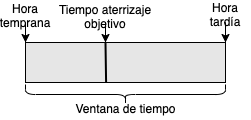
\includegraphics[width=6cm]{ventanadeTImepo.png}
    \caption{Ventana de tiempo de aterrizaje}
\end{figure} 

Más adelante en la definición de las variables y restricciones se puede observar las penalizaciones cuando un avión aterriza antes o después de su tiempo objetivo.

\subsection{Objetivos}
Como se puede observar explícitamente en lo expuesto en los primeros párrafos del punto anterior, el resolver el problema de ALSP tiene como principales objetivos:
\begin{itemize}
    \item Reducir la congestión de los aeropuertos.
    \item Minimizar costos de las aerolíneas.
    \item Encontrar una calendarización óptima de una secuencia de aterrizaje.
    \item Minimizar el tiempo ocioso de un avión en el aeropuerto.
    \item Minimizar el costo de no respetar los tiempos óptimos de aterrizaje.
\end{itemize}
\subsection{Variables}
\begin{itemize}
    \item Tiempo de aterrizaje asociado a un avión.
    \item Que tan pronto aterriza el avión antes del tiempo de aterrizaje (Grado de antelación).
    \item Que tan pronto aterriza el avión después del tiempo de aterrizaje.(Retraso del aterrizaje)
    \item Variables binarias asociadas para saber si un avión aterriza antes que otro, si un avión aterriza en una determinada pista y si dos aviones aterrizan en la misma pista.
\end{itemize}
\subsection{Restricciones}
Como se mencionó ALSP debe satisfacer diferentes restricciones, las cuales se pueden clasificar como:
\begin{itemize}
    \item \textbf{Restricciones Duras:} 
    \begin{itemize}
        \item El aterrizaje de cada avión debe encontrarse dentro de los límites de la ventana de tiempo asociado a este.
        \item Se debe respetar la separación entre el aterrizaje de un avión y el aterrizaje de todos los aviones sucesivos.
        \item Todos los aviones deben aterrizar.
        \item Todo avión debe aterrizar solo en una pista.
    \end{itemize}
    \item \textbf{Restricciones Blandas:}
    \begin{itemize}
        \item Se espera que los aterrizajes se realicen en un tiempo de aterrizaje esperado. De lo contrario, existirá una  penalización. 
    \end{itemize}
\end{itemize}
Como se señaló anteriormente cada avión debe aterrizar entre una ventana de tiempo determinada, teniendo un tiempo esperado de llegada que de no cumplirlo podría provocar retrasos en la planificación general de aterrizaje del aeropuerto, atrasar vuelos, generar una cola de espera entre los aviones que sobrevuelan en el aeropuerto esperando así se pueda desocupar la pista de aterrizaje. Las causas recién mencionadas son las principales de producir un aumento en la congestión y trafico dentro del aeropuerto, es por esto que se busca penalizar a cada avión que aterricé antes o después de su tiempo esperado.\\


\subsection{Dificultades detectadas}

Dentro de los principales factores que determinan el rendimiento y eficiencia de las pistas de aterrizaje se encuentra la separación requerida entre los aterrizajes y despegues de los aviones \cite{article1}. Debido a la alta complejidad que esto implica es muy difícil encontrar una solución óptima en la mayoría de los casos.

Al aumentar considerablemente las restricciones y el número de variables, también se ve afectado el espacio de las posibles soluciones, lo cual presenta este problema como \textbf{NP-hard} \cite{HybridAyudante}, es decir, que para su solución se requiere un esfuerzo computacional que crece exponencialmente al aumentar el tamaño de este, no admitiendo soluciones exactas eficientes.

Es importante mencionar que el número de vuelos, tanto de pasajeros como de aerolíneas de carga siguen aumentando en los últimos años \cite{HybridAyudante}, haciendo cada vez más complejo la resolución de este tipo de problemas.
\subsection{Variantes de ALSP}
Dentro de la literatura actual no se encuentran muchas variantes del presente problema, pero si se logra identificar algunas variaciones al momento de plantear la definición y objetivo de este, teniendo principalmente:
\begin{itemize}
    \item \textbf{Variación en cantidad de pistas de aterrizaje:} El aumentar la cantidad de pistas de aterrizaje hace que el problema crezca, tratando de atender la problemática de la forma más realista. Se destacan los siguientes artículos, donde podemos encontrar similitudes respecto al planteamiento de cada problema.
    \begin{itemize}
        \item \textbf{Una sola pista de aterrizaje:}
        \begin{itemize}
            \item \textit{"Solving Dynamic Single-Runway Aircraf Landing problems with extremal Optimization."}\cite{SingleRunway}, dicha representación unimodal se utiliza para implementar un algoritmo determinista que optimiza las líneas de tiempo.
        \end{itemize}
        
        \item \textbf{Múltiple pistas de aterrizaje:} Algunos articulos que utilizan múltiples pistas de aterrizajes:
        \begin{itemize}
            \item \textit{"Hybrid algorithms for the multiple runway aircraft landing problem"}\cite{HybridAyudante}.
            \item \textit{"\text{A} hybrid metaheuristic for multiple runways aircraft landing problem based on bat algorithm"}\cite{multiRunway}.
        \end{itemize}  

    \end{itemize}
    \item \textbf{Asignación dinámica:} El problema a estudiar en este articulo es un caso estático, sin embargo, existe su variante dinámica donde las decisiones sobre los tiempos de aterrizaje de los aviones se toman a medida que pasa el tiempo y la situación cambia, es decir, los aviones aterrizan, aparecen nuevos aviones, entre otros. \cite{article1}. Algunas de las literaturas que aplican modelos para esta variantes son:
    \begin{itemize}
        \item \textit{"Displacement problem and dynamically scheduling aircraft landings”} \cite{BeasleyDinamic}.
        \item \textit{"The Dynamic Scheduling of Aircraft in the Near Terminal Area"} \cite{Dear1976}.
    \end{itemize}
   
\end{itemize}

\newpage
\section{Estado del Arte}

\subsection{Origen y principales métodos utilizados en su resolución}

Es en el año 1959 en un artículo publicado por Alfred Blumstein \cite{Blumstein1959} donde por primera vez se estimó la capacidad de servicio de una pista de aterrizaje restringida por criterios de separación tantos espaciales como temporales. Más tarde, durante la últimas tres décadas, ha existido una gran variedad de estudios respecto a la optimización de la capacidad de los aeropuertos, donde se destaca por primera vez a Dear, R (1976)\cite{Dear1976} quien presenta un problema de optimización de múltiples objetivos buscando minimizar el retraso en un entorno dinámico con una única pista de aterrizaje, de esta formulación se destaca el concepto de \textit{Constrained Position Shifting} (CPS), cuya restricción busca que cada avión debe aterrizar dentro de un número de posiciones prefijadas (MPS) en una secuencia FCFS (First Come First Server).

Más tarde comienza aparecer uno de los más mencionados autores en la literatura asociada con ALSP, Beasley, quien en el año 2000 \cite{article1} junto a compañía, presentaron una heurística para resolver el problema dentro de un contexto estático considerando una única y múltiples pistas de aterrizajes, llamada \textbf{Heuristic Upper bound and Restarting}, teniendo:
\begin{itemize}
    \item \textbf{Upper bound:} Se busca encontrar un valor $Z_{ub}$ de límite superior en la solución óptima del problema, para poder ajustar las ventanas de tiempo para cada avión. Este nuevo límite superior busca a la vez reducir la búsqueda a un árbol LP-Based.
    \item \textbf{Restarting:} Al utilizar la heurística mencionada anteriormente, se obligó a reiniciar el problema cada vez que se encontraba una solución factible mejorada, encontrando una nueva solución en un tiempo menor a P (número de aviones) segundos después de comenzar la búsqueda del árbol.
\end{itemize}


Beasley et al. (2001) \cite{article2Europa} propusieron un algoritmo genético basado en poblaciones, el proceso consistía en seleccionar una solución inicial y realizar los pasos correspondientes de selección, combinación, mutación y evaluación con el fin de encontrar a los padres que continuarán en la siguiente iteración. La función de evaluación es no linear y tiene como objetivo privilegiar un aterrizaje previo al horario esperado y castigar el caso contrario.
Posteriormente, Beasley et al. (2004) \cite{BeasleyDinamic} presentaron una nueva formulación basada en Beasley et al. (2001), pero esta vez considerando un entorno dinámico, por lo cuál su objetivo era minimizar el desplazamiento del problema dentro de este nuevo ambiente. Utilizaron la misma metaheurística de algoritmo genético basado en poblaciones, pero modificando etapas con el fin de no entrar en el campo de soluciones infactibles, además de agregar la opción de elección de pista de aterrizaje. Los resultados computacionales los presentaron de acuerdo a instancias de 500 aviones y 5 pistas de aterrizaje.

Por su parte, Bencheikh et al. (2009) propusieron un método híbrido para resolver el problema dentro de un entorno estático y múltiples pistas de aterrizaje. El método combina dos metaheurísticas;
algoritmos genéticos y algoritmo de colonia de hormigas. \textbf{El algoritmo de colonia de hormigas} es utilizado para generar una solución inicial factible para el algoritmo genético, la formulación de este algoritmo se basa en el comportamiento que tienen en la vida real las diversas hormigas que vagan de manera aleatoria, al azar y que una vez encuentran comida regresan dejando feromonas, formando un camino que con el paso del tiempo las demás hormigas seguirán ya que se guiarán por el rastro dejado, es así, que bajo esta lógica, el algoritmo resulta como una técnica probabilística (basado en un calculo guiado por las "feromonas") para solucionar problemas de optimización, permitiendo reducir el espacio de búsqueda de las posibles soluciones lo que para el algoritmo genético provocará una alta probabilidad de encontrar buenas soluciones y de calidad de manera más rápida. Los resultados experimentales demostraron que iniciar con una solución obtenida mediante colonia de hormigas entrega muchos mejores resultados que mediante una solución inicial aleatoria, además, el método híbrido logra alcanzar el óptimo o estar muy cercano a él en la mayoría de las instancias. Los autores enfocaron sus próximos desafíos en adaptar el método para obtener mejores resultados en instancias grandes y considerar un entorno dinámico en vez de estático.

\subsection{Tendencia}
Resumiendo lo expuesto en la sección anterior se ha generado la siguiente tabla en la cual se puede observar cada articulo mencionado con su correspondiente entorno, $N$º de pistas de aterrizaje y el tipo de modelo utilizado.

\begin{table}[h]
\begin{tabular}{|l|l|l|l|l|}
\hline
\textbf{Artículo }               & \textbf{Modelo}                                           & \textbf{Entorno}  & \begin{tabular}[c]{@{}l@{}}\textbf{Nº pistas de} \\ \textbf{aterrizaje}\end{tabular} & \textbf{Función Objetivo}                                                                                                                 \\ \hline
Dear, R. (1976) \cite{Dear1976}       & \begin{tabular}[c]{@{}l@{}}DP\\ CSP\end{tabular} & Dinámico & Única                                                              & Minimizar el máximo retraso.                                                                                                     \\ \hline
Beasley et al. (2000) \cite{article1}   & MIP                                              & Estático & \begin{tabular}[c]{@{}l@{}}Única / \\ múltiples\end{tabular}       & \begin{tabular}[c]{@{}l@{}}Minimizar el costo total, \\ relacionado con la desviación \\ de su tiempo objetivo\end{tabular}      \\ \hline
Beasley et al. (2001) \cite{article2Europa}   & MIP                                              & Estático & Única                                                              & \begin{tabular}[c]{@{}l@{}}Privilegiar un aterrizaje previo \\ al horario esperado y castigar \\ el caso contrario.\end{tabular} \\ \hline
Beasley et al. (2004) \cite{BeasleyDinamic}  & \begin{tabular}[c]{@{}l@{}}MIP\\ DP\end{tabular} & Dinámico & Múltiples                                                          & \begin{tabular}[c]{@{}l@{}}Minimizar el costo total, \\ relacionado con la desviación \\ de su tiempo objetivo\end{tabular}      \\ \hline
Bencheikh et al. (2009) \cite{HybridAyudante} & JSP                                              & Estático & Múltiples                                                          & \begin{tabular}[c]{@{}l@{}}Minimizar el costo total de \\ penalización\end{tabular}                                              \\ \hline
\end{tabular}

\caption{Tabla clasificación de los artículos expuestos }
\label{tablita}
\end{table}
\textbf{Obervación:} CSP: \textit{Constrained Position Shifting}, MIP: \textit{Mixed Integer
Porgramming Model}, DP: \textit{Displacement problem}, JSP: \textit{Job Shop Scheduling Model}\\

El cuadro \ref{tablita} deja en evidencia como el modelado MIP ha sido uno de los más utilizados, esto debido a principalmente a que el usar variables binarias de decisión se permite relacionar la decisión de la hora de aterrizaje de cada avión respetando los tiempos de separación en el aterrizaje con optimizar el tiempo objetivo.

Independiente de las variaciones respecto al Nº de pistas de aterrizaje, la mayoría de los problemas buscan cumplir el objetivo de minimizar el costo total de penalización, lo cual traducido para las aerolíneas significará menor congestión y un transito más fluido en su entrada y salida de aviones. El usar múltiple pistas agregará más restricciones, haciendo crecer más aún la dificultad computacional de resolver el problema, pero esperando encontrar una solución más factible y óptima en la vida real.

En la actualidad la mayoría de los artículos se basan en los resumidos en la tabla \ref{tablita}, buscando mejorar la precisión con la que se puede encontrar una solución factible, destacándose el uso de métodos híbridos y exactos.
A continuación se presenta una tabla que compara tres artículos del último tiempo.

\begin{table}[h]
\centering
\begin{tabular}{|l|l|l|l|l|}
\hline
Artículo                & \textbf{Metodología} & \textbf{Entorno} & \textbf{\begin{tabular}[c]{@{}l@{}}Nº pistas de \\ aterrizaje\end{tabular}} & \textbf{Modelo} \\ \hline
Awasthi et al. (2013) \cite{2013}   & Exacto               & Estático         & \begin{tabular}[c]{@{}l@{}}Única/\\ Multiples\end{tabular}                  & MIP             \\ \hline
Lieder et al. (2015) \cite{2015}    & Exacto               & Estático         & Múltiples                                                                   & DP              \\ \hline
Salehipour et al.(2020) \cite{SALEHIPOUR2020179}& Exacto               & Diámico          & \begin{tabular}[c]{@{}l@{}}Única/\\ Multiples\end{tabular}                  & DP              \\ \hline
\end{tabular}
\caption{Tabla clasificación de los últimos artículos métodos exactos.}
\label{tablita2}
\end{table}

Se destaca el articulo más reciente de Salehipour (2020) \cite{SALEHIPOUR2020179}, en donde los autores proponen un nuevo método heurístico para resolver el problema considerando una única pista y múltiples pistas de aterrizaje. El método consiste en, inicialmente se genera una secuencia inicial construida de acuerdo a los horarios de llegada de los aviones, posicionando en orden creciente, es decir, partiendo por aquellos con una llegada más temprana. Para el caso de múltiples pistas, un avión se posiciona en una segunda pista solo cuando no es posible que aterrice en la primera en su tiempo esperado. Luego, se selecciona una porción pequeña de los aviones, para los cuales se relaja y optimiza su posición en la secuencia mediante el uso de un método exacto, similar a lo expuesto por \cite{article1} (los aviones fuera de esta porción quedan sin modificación). Se repite el mismo procedimiento hasta que se llega a una condición de término (tiempo de ejecución o máximo de iteraciones).

\subsection{Resultados a la fecha}

Se realiza la comparación de los resultados de los últimos tres artículos presentes en la tabla \ref{tablita2}, para 13 instancias con 1 pista de aterrizaje obteniendo:

\begin{table}[h]
\centering
\begin{tabular}{|l|l|l|}
\hline
Método                  & \textbf{\# Mejores soluciones} & \textbf{\% Mejor solución} \\ \hline
Salehipour et al.(2020) \cite{SALEHIPOUR2020179} & 10                             & 76.92                      \\ \hline
Awasthi et al. (2013) \cite{2013}   & 8                              & 69.23                      \\ \hline
Lieder et al. (2015) \cite{2015}   & 11                             & 61.54                      \\ \hline
\end{tabular}
\caption{Resumen de los métodos de solución para resolver las instancias de referencia con 1 con una pista de aterrizaje. \cite{SALEHIPOUR2020179}}
\end{table}

Así mismo se hizo la comparación para \textbf{múltiples pistas de aterrizajes}, obteniendo, presentando 36 instancias de un conjunto para múltiples pistas, obteniendo:

\begin{table}[h]
\centering
\begin{tabular}{|l|l|l|}
\hline
Método                  & \textbf{\# Mejores soluciones} & \textbf{\% Mejor solución} \\ \hline
Salehipour et al.(2020) & 34                             & 94.44                      \\ \hline
Awasthi et al. (2013) \cite{2013}  & 29                             & 80.56                      \\ \hline
Lieder et al. (2015) \cite{2015}   & 25                             & 69.44                      \\ \hline
\end{tabular}
\caption{Resumen de los métodos de solución para resolver instancias para múltiples pistas de aterrizajes.\cite{SALEHIPOUR2020179}}
\end{table}


Basta destacar que los conjuntos de instancias presentados en estos resultados corresponden al conjunto 1 presente y explicado en \cite{SALEHIPOUR2020179}.





\newpage
\section{Modelo Matemático}
Se presenta a continuación una formulación lineal entera mixta, basado en lo expuesto por Beasley en \cite{article1}, cuyo modelo en un principio solo utiliza una pista de aterrizaje, pero luego más adelante se presenta una heurística eficaz para el problema con cualquier número de pistas, complementando y teniendo en cuenta el entorno estático sobre el cual se define el problema, se tiene lo siguiente.\\

\subsection{Definición de parámetros para modelo ALSP}
\begin{table}[h]
\begin{tabular}{ll}
$P:$  & Número de aviones.  \\
$N:$  & Número de pistas de aterrizaje.  \\
$E_i:$ & Tiempo más temprano de aterrizaje para el avión $i$.\\
$L_i:$ & Tiempo más tardío de aterrizaje para el avión $i$.\\
$T_i:$ & Tiempo objetivo de aterrizaje para el avión $i$.\\
$[E_i,L_i]:$ & Ventana temporal del avión $i$.\\
${S}_{ij}:$ & Tiempo de separación requerido entre el aterrizaje del avión $i$ \\
& y el aterrizaje del avión $j$ en una misma pista de aterrizaje.\\
$g_i:$ & Coste de penalización ($\geq 0$) por unidad de tiempo si el avión aterriza antes que $T_i$.\\
$h_i:$ & Coste de penalización ($\geq 0$) por unidad de tiempo si el avión aterriza después que $T_i$.
\end{tabular}
\end{table}

Hay que destacar que cuando se habla del problema como un caso estático \cite{article1}, el número de aviones $P$ y la información asociada a cada uno de ellos es informada al comienzo.

\subsection{Variables}

\begin{table}[h]
\begin{tabular}{ll}
$x_i = $  & Tiempo de aterrizaje del avión $i$\\
$\alpha_i = $ & Indica el grado de antelación del aterrizaje del avión $i$ respecto $T_i$\\
$\beta_i = $ & Indica el retraso del aterrizaje del avión $i$ respecto $T_i$
\end{tabular}
\end{table}

$$
\delta_{i j}=\left\{\begin{array}{c}1 \quad \text { si el avión } i \text{ aterriza antes que el avión } j. \\ 0 \quad \text { en otro caso. }\end{array}\right.
$$

$$
{y}_{jr}=\left\{\begin{array}{c}1 \quad \text { si el avión } j \text{ aterriza en la pista } r \quad \forall (i \in P; r \in N) \\ 0 \quad \text { en otro caso. }\end{array}\right.
$$

$$
{z}_{ij}=\left\{\begin{array}{c}1 \quad \text { si el avión } i \text{ y } j \text{ aterrizan en la misma pista }. \forall(i,j \in P; i \neq j) \\ 0 \quad \text { en otro caso. }\end{array}\right.
$$
\subsection{Función Objetivo}
El coste que se presenta corresponde al coste adicional cuando el aterrizaje no es en el tiempo $T_i$. Teniendo:
$$
\begin{array}{ll}\alpha_{i}=\max \left(0, T_{i}-x_{i}\right) & i=1, \ldots, P \\ \beta_{i}=\max \left(0, x_{i}-T_{i}\right) & i=1, \ldots, P\end{array}
$$
\\
Así según lo recién expuesto la función objetivo a minimizar corresponde a:\\
\begin{equation}
    \min \sum_{i=1}^{P} \alpha_i g_i + \beta_i h_i
    \label{fo1}
\end{equation}
La  ecuación  (\ref{fo1}) busca minimizar la penalización de la desviación respecto al tiempo objetivo utilizando los costes de $g_i$ y $h_i$.
\subsection{Restricciones}

\begin{equation}
E_{i} \leq T_{i} \leq L_{i}, \quad \forall i \in P ; i \neq j
\label{r1}
\end{equation}

\begin{equation}
\delta_{i j}+\delta_{j i} \leq 1, \quad \forall i, j \in P
\label{r2}
\end{equation}

\begin{equation}
\sum_{r=1}^{N} y_{i r}=1, \quad \forall i \in P ; r \in N
\label{r3}
\end{equation}

\begin{equation}
z_{i j}=z_{j i}, \quad \forall i, j \in P ; i \neq j
\label{r4}
\end{equation}

\begin{equation}
z_{i j} \geq y_{i r}+y_{j r}-1, \quad \forall i, j \in P ; i \neq j
\label{r5}
\end{equation}

\begin{equation}
x_{j} \geq x_{i}+S_{i j} \cdot z_{i j}+\left(L_{i}+S_{i j}-E_{j}\right) \cdot \delta_{j i}, \quad \forall i, j \in P; i \neq j.
\label{r6}
\end{equation}

\begin{equation}
\alpha_{i} \geq T_{i}-x_{i}, \quad \forall i \in P
\label{r7}
\end{equation}

\begin{equation}
0 \leq \alpha_{i} \leq T_{i}-E_{i}, \quad \forall i \in P
\label{r8}
\end{equation}

\begin{equation}
\beta_{i} \geq x_{i}-T_{i}, \quad \forall i \in P
\label{r9}
\end{equation}

\begin{equation}
0 \leq \beta_{i} \leq L_{i}-T_{i}, \quad \forall i \in P
\label{r10}
\end{equation}

\begin{equation}
x_{i}=T_{i}-\alpha_{i}+\beta_{i}, \quad \forall i \in P
\label{r11}
\end{equation}

\begin{equation}
\delta_{i j}, y_{i j}, z_{j r}, \quad \forall i, j \in P ; i \neq j
\label{r12}
\end{equation}

\begin{itemize}
    \item (\ref{r1}) asegura que el tiempo de aterrizaje para cada avión debe estar comprendido en el intervalo de su ventana temporal [$E_i$, $L_i$].
    \item (\ref{r2}) verifica que para cada par de avión, un avión aterrice antes que otro, ya sea el avión $i$ antes $j$ o viceversa.
    \item (\ref{r3}) Se encarga de que todo avión aterrice solo en una pista. 
    \item La restricción (\ref{r4}) verifica si los aviones $i$ y $j$ aterrizan en la misma pista. Así mismo (\ref{r5}) fuerza a la variable $z_{ij}$ a tomar el valor de 1, si los aviones $i$ y $j$ aterrizan en la misma pista.
    \item La restricción (\ref{r6}) se encarga de hacer cumplir la separación temporal, que considera dos casos donde $\delta_{ij}$ = 1 significa que el avión $i$ aterrizó antes que $j$, por lo que $\delta_{ji}$ = 0, lo cual fuerza a la separación ($x_j \leq  x_i + S_{ij}$), en caso contrario si $\delta_{ij}$ = 0 $\Rightarrow \delta_{ji} = 1$ provocando que  $x_j \geq$ ($L_i$ + $S_{ij}$ - $E_j$) cuyo número será un negativo grande, lo que que garantizará finalmente una contradicción lógica.
    \item Las restricciones (\ref{r7}) y (\ref{r8}) determinan los valores limites que puede tomar la variable $\alpha_i$, así mismo las restricciones (\ref{r9}) y (\ref{r10}) indican los valores limites para $\beta_i$
    \item La restricción (\ref{r11}) indica la relación existente entre el tiempo de aterrizaje y las variables $\alpha_i$ y $\beta_i$, correspondiendo a la penalización asociada.
    \item Finalmente la restricción (\ref{r12}) comprende la naturaleza de las variables binarias.
\end{itemize}

\section{Representación}
Para llevar a cabo la resolución del presente problema se utilizaron las siguientes estructuras:
\subsection{Para la solución:}
Se utilizó un vector llamado \textbf{solucionActual} de largo \textbf{$P$} (número de aviones), donde cada espacio $i$ corresponde a un avión y su contenido $solucionActual[i]$ será el tiempo de aterrizaje $x_i$ asignado para él. Dicha estructura se puede observar a continuación:

\begin{figure}[h]
    \centering
    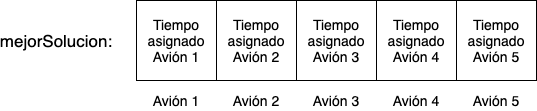
\includegraphics[width=10cm]{solucionVector.png}
    \caption{Representación gráfica del vector solucionActual.}
    \label{fig:vectorSolucion}
\end{figure}

El presente vector se va actualizando cada vez se encuentra una nueva solución con mejor evaluación en la función objetivo.

\subsection{Para los tiempos de separación entre aviones:}
Se construyó una matriz de $PxP$ para representar la separación entre los tiempos de aterrizaje que se debe respetar entre el avión $i$ y el avión $j$, obteniendo:
\begin{center}
    \begin{equation*}
    \begin{pmatrix}
    S_{00} & S_{0j} & \cdots & S_{0p}\\
    S_{i0} & S_{ij} & \cdots & S_{ip}\\
    \vdots & \vdots & \ddots & \vdots\\
    S_{p0} & S_{pj} & \cdots & S_{pp}\\
    \end{pmatrix}
\end{equation*}
con   $i$ $\wedge$ $j$ $\in [0,p]$
\end{center}

A dicha matriz se accede en cada verificación del dominio de los aviones a instanciar un tiempo, validando la restricción de separación temporal.\\

\subsection{Para almacenar los datos de cada avión:}
Siguiendo la lógica de la construcción del vector solución, se creó un \textbf{vector de aviones}, donde cada elemento corresponde a un \textbf{struct Avion} el cual almacena los datos la información del avión del indice $i$, detallado de la siguiente manera:
\begin{itemize}
    \item \textbf{struct Avion}: Contiene los tiempo $E_i$, $T_i$ y $L_i$, las penalizaciones $g_i$ y $h_i$, y un vector \textbf{dominio} donde se almacena el dominio del avión $i$ que en un comienzo irá desde $E_i$ hasta $L_i$.

\end{itemize}

\subsection{Otras estructuras:}
\begin{itemize}
    \item \textbf{struct Solucion}: Se utiliza para almacenar la información de la mejor solución actual, almacenando el vector de los tiempos asignados para cada avión, el costo de esta solución y el tiempo que se demoró el algoritmo en encontrarla.
    \item \textbf{struct ContadorInstancias}: Utilizada para almacenar el nombre de la instancia actual, la cantidad de variables instanciadas, el número de chequeos y de retornos ocurridos en el algoritmo.
    
\end{itemize}

\section{Descripción del algoritmo}

La solución del presente problema fue realizada mediante Forward Checking (FC) + Graph back-jumping (GBJ), donde FC se encargó de la \textbf{exploración} del espacio de búsqueda para poder instanciar las variables y \textbf{GBJ} en la \textbf{intensificación} de la solución guiando el retroceso del algoritmo a la última variable instanciada.

Forward Checking es un algoritmo del tipo Look-ahead basado en Backtracking (BT), es decir, explorará todas las posibles combinaciones de las variables sobre las que se itera. La forma de desarrollar FC puede ser tanto iterativamente como recursiva, por lo que en este punto se busca sacar ventaja  en cuanto a extensión de lo que premia un algoritmo recursivo. A diferencia de BT tiene una gran ventaja, que consiste en que antes de instanciar la siguiente variable (próximo nivel del arbol), se filtra el dominio de las próximas variables según las restricciones del problema, lo que se considera como mirar hacia adelante (Look-ahead)\\

El filtrado del dominio en este problema esta basado principalmente en la restricción de respetar la separación en los tiempos de aterrizaje de cada avión con los demás. Este retorno guiado por el grafo (GBJ) a modo grueso consistió en volver a la variable más cercana conectada al nodo del cual se tiene un conflicto (principalmente que posee o más adelante hay un dominio vacío, es decir, que una variable no puede tomar seguir instanciándose).\\

Basta destacar que la realización del presente algoritmo se utilizó una única pista de aterrizaje, lo cual satisface la restricción (\ref{r3}) del modelo matemático. Al mismo tiempo el dominio de cada avión se estableció dentro del rango [$E_i$, $L_i$] satisfaciendo así la restricción (\ref{r1}) \\
De esta manera, el algoritmo parte instanciando el primer avión con el primer valor de su dominio (en un principio $E_i$), según el orden que viene entregado en la instancia, al realizar esto se actualizan todos los dominios de los (p-1) aviones siguientes conservando solo los valores que siguen siendo válidos de acuerdo a las restricciones del problema, donde la principal restricción utilizada para filtrar estos dominios consistió en verificar en la matriz de separación que se respete la separación entre los tiempos de aterrizajes de los aviones (restricción (\ref{r6}), quedando de manera implícita las demás restricciones dado que el orden de instanciación obligará que dicho avión aterrice antes o después de otro. Para el segundo avión se realiza exactamente el mismo proceso, filtrando nuevamente los dominios para los siguiente (p-2 aviones). Como el proceso continua de igual manera para los siguientes aviones, el algoritmo realiza recursión en la instanciación de cada avión, devolviéndose solo en 2 condiciones; si se llega al último avión y por ende a \textbf{una solución}, o  si se encuentra un dominio vacío para alguno de los aviones que faltan por instanciar. Para la primera opción, se procede a evaluar la solución en la función objetivo del problema (satisfaciendo al mismo tiempo las restricciones (\ref{r7}) a la (\ref{r11}) que están explicitas en como se escribió la FO en el código),la cual otorgará el costo de esta, dicho costo será utilizado para comprobar si es o no la mejor solución encontrada hasta el momento. En cualquiera de las dos condiciones explicadas anteriormente, el algoritmo retorna al último elemento previamente instanciado (GBJ), asignándole el siguiente valor correspondiente de su dominio y continuar el proceso desde ahí.\\

A continuación se puede observar el pseudocódigo del algoritmo descrito, el cual contempla las llamadas recursivas a la función \textbf{ForwardChecking}, comenzando desde la primera instanciación, con dominio inicial desde [$E_0$, $L_i$].\\

\begin{algorithm}[h]
\caption{Forward Checking + GBJ}\label{euclid}
\begin{algorithmic}[1]
    \BState $p \gets$ cantidad de aviones.
    \BState $Aviones \gets$ vector de tamaño p que contiene los aviones del problema.
    \State $matrizSeparacion \gets$ contiene las separaciones requeridas entre aviones.
    \BState $instanciaActual \gets 0$ posición de la instancia actual, se comienza con la primera.
    \BState $solucion \gets$ vector con los tiempos asignados.
    \State $solucion[0] \gets E_0$.
    \State $costoSolucion \gets$ inf.
    \State $dominioActual \gets$ 0.

    \Procedure{ForwardChecking}{Aviones, instanciaActual, solucion, dominioActual}
    \State $valorInstancia \gets solucion[instanciaActual]$
    \If {instanciaActual == p-1}
    \State $costoActual \gets$ evaluarSolucion(solucion)
    \If {$costoActual < costoSolucion$}
    \State $costoSolucion \gets costoActual$
    \EndIf
    \State \textbf{return 1}
    \EndIf
    \State $AvionesFiltrados \gets filtrarDominios(Aviones, matrizSeparacion, valorInstancia)$ 
    
    \If{existe algun dominio vacio?}
    \State \textbf{return 0}
    \Else 
    \For{i= 0 to i= len(DominioAvionesfiltrados[instanciaActual])}
    \State ForwardChecking(AvionesFiltrados, instanciaActual+1 solucion,dominioActual)
    \EndFor
    \State \textbf{return 1}
    \EndIf
    
    
    
    \EndProcedure
    
    \For{ i = 0 to i = len(DominioAviones[0])}
    \State solucion[0] = Aviones[0].dominio[i];
    \State ForwardChecking(Aviones, instanciaActual solucion,dominioActual)
    \EndFor
    
    \end{algorithmic}
\end{algorithm}


\section{Experimentos}
El proceso de experimentación se llevó a cabo en un dispositivo de las siguientes características:\\

\begin{table}[h]
\centering
\begin{tabular}{|l|l|}
\hline
\multicolumn{2}{|c|}{\textbf{Dispositivo utilizado}} \\ \hline
\textbf{Procesador:}      & Ryzen 5 3600 3.9 OC      \\ \hline
\textbf{RAM:}             & 2x 8GB 3200 MHz          \\ \hline
\textbf{Gráfica:}         & Asus GTX 1050 2GB        \\ \hline
\textbf{HDD:}             & 2x 500GB                 \\ \hline
\textbf{SSD:}             & Evo 860 1TB              \\ \hline
\end{tabular}
\end{table}

El problema al ser resuelto por una técnica de búsqueda completa se definió de forma general que la cantidad de pistas de aterrizajes a considerar sería siempre 1 ($N$= 1).\\

La definición de los parámetros restantes se realiza al momento de leer las instancias a evaluar, cada instancia contempla el número de aviones $P$, sus tiempos $E_i$, $L_i$ y $T_i$, las separaciones de tiempos de aterrizaje $S_{ij}$, y las penalizaciones $g_i$ y $h_i$, las cuales fueron almacenadas en nuestro modelo tal como se describe en la sección de representación.

Las instancias utilizadas para la experimentación fueron las entregadas por el ayudante y se pueden encontrar en la carpeta del proyecto. El formato de entrada de cada instancias se detalla de la siguiente forma:
\begin{figure}[h]
    \centering
    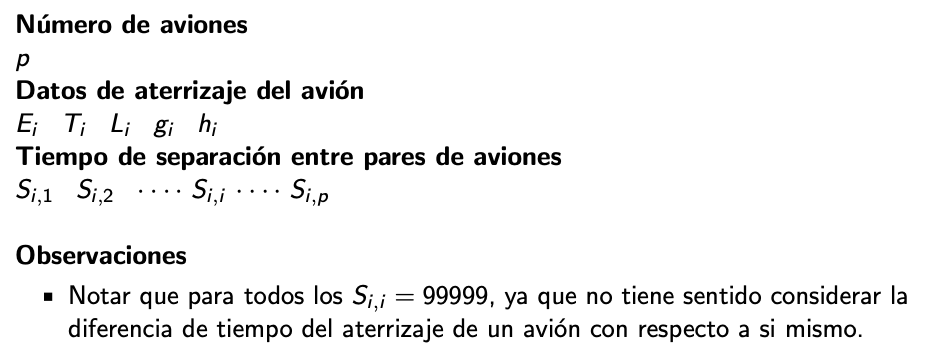
\includegraphics[width=13cm]{detalleInstancia.png}
\end{figure}

Para verificar la correcta implementación del algoritmo descrito, se creó una nueva instancia de prueba (\textit{airland$\_$test.txt}), la cual se encuentra junto a las demás instancias en la carpeta del proyecto. Con esta instancia se obtuvo una solución global en un tiempo de 2.04646 [seg], se detalla el resultado completo en la siguiente sección.\\
El objetivo principal de realizar la experimentación es encontrar un óptimo global para cada instancia con el fin de demostrar el correcto funcionamiento del algoritmo FC+GBJ, sin embargo, al ser una búsqueda completa se espera un alto tiempo de ejecución, por lo que más adelante se plantea una forma para poder obtener la mejor solución hasta el momento.\\

En total se probaron 14 instancias, considerada la de test mencionada anteriormente. En primer lugar se ejecutó la instancia \textit{airland1.txt} y \textit{airland2.txt} por un periodo de 38 horas, 11 minutos y 49 seg, sin obtener una solución final (que finalizara el algoritmo), por ende, no se sabe cual fue la mejor solución encontrada hasta ese momento, sin embargo, se imprimió el costo de la mejor solución y el tiempo en el que fue encontrada, obteniéndose: 

\begin{table}[h]
\centering
\begin{tabular}{|l|l|l|}
\hline
\multicolumn{3}{|c|}{\textbf{Primeras pruebas - Tiempo total : 136.915 {[}s{]}}} \\ \hline
\textbf{Nombre instancia}     & \textbf{Costo}     & \textbf{Tiempo {[}s{]}}     \\ \hline
airland1.txt                  & 3650               & 0,002247                    \\ \hline
airland2.txt                  & 8370               & 100.376,2                   \\ \hline
\end{tabular}
\end{table}

Es importante observar de la tabla recién expuesta que la mejor solución encontrada durante todo el tiempo extenso de ejecución ocurrió en los primeros segundos y luego no pudo encontrar una mejor, lo que se traduce en que la posible solución de esta instancia se encuentra variando las instanciaciones de las primeras variables (aviones). Pensando en una futura experimentación se podría establecer que si no se encuentra una nueva solución luego de un tiempo de ejecución \textit{X} se proceda a variar las primeras instanciaciones para llegar más rápido al óptimo global, sin embargo, este tiempo debe ser bien calculado para no perder parte importante de la información obtenida, por que por ejemplo la instancia \textit{airland2.txt} mostró diversas mejoras de soluciones a lo largo del tiempo, siendo la penultima en un tiempo de 86.603,4 [seg] y la última en un tiempo de 100.376,4 [seg], lo cual es una variación de 13.773 [seg], este tiempo podría ser utilizado como un tiempo limite para aplicar un nuevo movimiento, pero solo para esta instancia, ya que las otras tienen un comportamiento independiente y distinto.\\ 

Dado lo ocurrido anteriormente (largo tiempo de ejecución del algoritmo con las instancias) se procedió a incorporar en el código el manejo del evento \textit{CTRL + C}, el cual al interrumpir la ejecución del algoritmo, se entrega la información de cual es la mejor solución encontrada hasta el momento, su costo, la cantidad de variables instanciadas, el número de chequeos y de retornos ocurridos en el algoritmo. Todo lo anterior además se almacena en un archivo de texto llamado \textit{solucion$\_$nombreInstancia.txt}, donde \textit{nombreInstancia} corresponde al nombre de la instancia que se está probando.

Se adjunta en la carpeta del proyecto una carpeta llamada \textit{[PAPER] Soluciones presentadas}, en la cual se puede observar los diversos archivos generados para cada una de las 14 instancias al interrumpir la ejecución del código en un tiempo de ejecución aproximado para la gran mayoría de 6 [horas].\\

El formato de salida al momento de interrumpir la ejecución del algoritmo se ejemplifica en la siguiente figura, que detalla lo obtenido al ejecutar la instancia \textit{airland1.txt} en un tiempo de 70931.7 [s].\\

\begin{figure}[h]
    \centering
    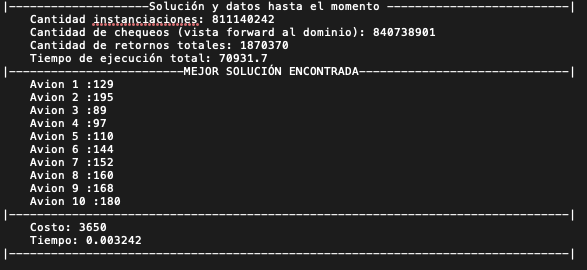
\includegraphics[width=14cm]{airland1.png}
    \caption{Lectura del archivo solucion$\_$airland1.txt}
    \label{fig:my_label}
\end{figure}

En base a lo anterior, el objetivo de la experimentación consistirá en encontrar al menos una solución del problema, en un tiempo mínimo de ejecución de 6 horas, para cada instancia, con el fin de poder analizar que ocurre en cada caso y dar cuenta de una idea más general de la eficiencia de este algoritmo. En la siguiente sección se presentan los resultados para las 14 instancias dispuestas.\\

\newpage
\section{Resultados}
Como se detalló en la sección anterior como primera experimentación para verificar y comprobar que se encuentra un óptimo global con el algoritmo implementado, se ejecutó este con la instancia de prueba \textit{airland$\_$test.txt}, obteniendo:\\
    %tabla test
    \begin{table}[h]
    \centering
    \begin{tabular}{|l|c|l|l|}
    \hline
    Avión          & 1                        & \multicolumn{1}{c|}{3} & \multicolumn{1}{c|}{2} \\ \hline
    Instante       & \multicolumn{1}{l|}{150} & 260                    & 280                    \\ \hline
    Costo          & \multicolumn{3}{c|}{150}                                                   \\ \hline
    Tiempo {[}s{]} & \multicolumn{3}{c|}{2,04646}                                               \\ \hline
    \end{tabular}
    \caption{Solución para la instancia \textit{airland$\_$test.txt}}
    \end{table}
    
Por otro lado, los mejores tiempos encontrados en un periodo de aproximadamente 6 horas para las instancias de la 2 a la 13 y 20 horas para la primera instancia, fueron los siguientes.

    %tabla 1exp
    \begin{table}[h]
    \centering
    \begin{tabular}{|l|l|l|l|}
    \hline
    \textbf{Nombre instancia} & \textbf{Costo solución} & \textbf{\begin{tabular}[c]{@{}l@{}}Tiempo mejor solución\\ encontrada {[}s{]}\end{tabular}} & \textbf{\begin{tabular}[c]{@{}l@{}}Tiempo interrupción \\ algoritmo {[}s{]}\end{tabular}} \\ \hline
    \textit{airland1.txt}     &        3.650                 &     0,003242                                                                                        &    70.931,7                                                                                       \\ \hline
    \textit{airland2.txt}     & 8.040                    & 24.487,5                                                                                     & 24.545,5                                                                                   \\ \hline
    \textit{airland3.txt}     & 21.270                   & 24.567,1                                                                                     & 24.573,5                                                                                   \\ \hline
    \textit{airland4.txt}     & 14.890                   & 1,165                                                                                       & 24.607,4                                                                                   \\ \hline
    \textit{airland5.txt}     & 21.590                   & 0,002                                                                                       & 24.609,4                                                                                   \\ \hline
    \textit{airland6.txt}     & 10.829                   & 0,003                                                                                       & 24.613,1                                                                                   \\ \hline
    \textit{airland7.txt}     & 5.871                    & 12.406,9                                                                                     & 24.670                                                                                     \\ \hline
    \textit{airland8.txt}     & 90.855                   & 24.342,9                                                                                     & 24.656,1                                                                                   \\ \hline
    \textit{airland9.txt}     & 40.197                   & 23.931,9                                                                                     & 24.009,9                                                                                   \\ \hline
    \textit{airland10.txt}    & 58.461                   & 11.281,1                                                                                     & 23.995,6                                                                                   \\ \hline
    airland11.txt             & 78.305                   & 13.471,2                                                                                     & 20.506,2                                                                                   \\ \hline
    airland12.txt             & 98.763                   & 20.246,3                                                                                     & 20.569                                                                                     \\ \hline
    ariland13.txt             & 182.921                  & 20.263,3                                                                                     & 20.595                                                                                     \\ \hline
    \end{tabular}
    \caption{Tiempos y costos de la mejor solución encontrada para cada instancia hasta el tiempo en que se interrumpió la ejecución del algoritmo.}
    \label{tablaSolucion1}
    \end{table}
    
Se puede observar en el cuadro \ref{tablaSolucion1} que para las instancias \textit{airland1.txt, airland5.txt, airland6.txt} la solución presentada corresponde a una obtenida en los primeros segundos de la ejecución del código, lo que confirma la poca eficiencia del algoritmo en cuestión y como se pudo observar en la sección anterior en un mayor tiempo de ejecución, tampoco se logra llegar a un mejor óptimo. Es en estos casos donde se puede aplicar un movimiento o variación de la técnica con el fin de encontrar el óptimo esperado en un menor tiempo.

También es importante señalar que independiente del tamaño de la instancia (Nº aviones e Intervalos de tiempo para cada avión) el algoritmo encuentra una solución en todas las instancias, y se confirma que el tiempo de cada una de estas dependerá netamente de como se vaya asignando los valores a las instancias.\\

A continuación se presenta la información general al momento de interrumpir la ejecución de cada instancia.\\
    %tablaNUMERO INSTANCIAS 
    \begin{table}[h]
    \centering
    \begin{tabular}{|l|l|l|l|}
    \hline
    \textbf{Nombre instancia} & \textbf{NºInstanciaciones} & \textbf{NºChequeos} & \textbf{Nº Retornos} \\ \hline
    \textit{airland1.txt}     &     811.140.242                       &      840.738.901                &           1.870.370            \\ \hline
    \textit{airland2.txt}     & 1.289.802.311                 & 1.128.507.132          & 6.173.863              \\ \hline
    \textit{airland3.txt}     & 1.006.065.879                 & 1.064.946.522          & 3.717.631              \\ \hline
    \textit{airland4.txt}     & 1.979.447.315                 & 1.852.443.474          & 4.640.831              \\ \hline
    \textit{airland5.txt}     & 1.532.180.609                 & 1.400.203.418          & 8.405.031              \\ \hline
    \textit{airland6.txt}     & 1.944.704.824                 & 1.833.238.033          & 67.982.228             \\ \hline
    \textit{airland7.txt}     & 592.739.123                  & 1.810.106.588          & 8.679.361              \\ \hline
    \textit{airland8.txt}     & 1.112.672.932                 & 1.127.163.524          & 2.453.482              \\ \hline
    \textit{airland9.txt}     & 392.358.212                  & 433.807.441           & 240.579               \\ \hline
    \textit{airland10.txt}    & 111.791.392                  & 141.100.397           & 68.419                \\ \hline
    airland11.txt             & 254.333.685                  & 317.594.093           & 156.945               \\ \hline
    airland12.txt             & 201.741.453                  & 275.198.473           & 129.351               \\ \hline
    ariland13.txt             & 24.484.939                   & 251.297.802           & 16.321                \\ \hline
    \end{tabular}
    \caption{Cantidad de instanciaciones, número de chequeos y retorno de cada instancia al momento de interrumpir la ejecución del algoritmo.}
    \end{table}
\\
\\
\\
Se observa que todas las cantidades de instanciaciones están en el orden de los millones, y los números de chequeos aproximadamente en la mitad de las pruebas superan el orden de los mil millones, lo cual comprueba que el algoritmo FC en su \textit{mirada hacia adelante} va filtrando el dominio de las posibles siguientes instanciaciones. Destaca dentro del número de retornos la instancia número 6, la cual posee 67.982.228 retornos, dicha cantidad es principalmente que en este caso existe una entrada recurrente a la condición de que si existe un dominio vacío en alguna de las variables y esto principalmente a que el valor $E_i$, $T_i$, $L_i$ del primer avión es 0. Viendo el comportamiento desde la instancia 8 a la 13 se observa una disminución de los número de retorno, lo que se asocia a la alta cantidad de aviones (variables) que hay que instanciar y el amplio intervalo de tiempo de aterrizaje que tiene cada uno, por lo que existen muchos posibles valores del dominio que se puede asignar a una variable antes de producirse un retorno.\\

Se incluye en el presente informe una sección de Anexo en la sección 11, donde se puede observar las soluciones encontradas para cada instanciación. La forma de presentar dicha solución es la descrita en la sección de representación como vector de solución donde cada espacio del vector representa un avión y el valor contenido en este el tiempo asignado de aterrizaje.

\section{Conclusiones}
Durante las últimas décadas se han realizado numerosos trabajos y avances sobre el problema ALSP y sus distintas derivadas, haciendo un barrido por distintos métodos exactos y heurísticas, en conjunto con combinaciones de ambos. Durante los primeros años del problema el desarrollo estaba enfocado en las versiones más simples del mismo, donde se consideraban entornos estáticos y una única pista de aterrizaje. Con el tiempo, y dado que la obtención de buenas soluciones era cada vez más recurrente, el problema fue ganando dificultad, agregando múltiples pistas y un contexto dinámico, en donde los tiempos de aterrizaje o la cantidad de aviones pueden variar con el tiempo. Dentro de todo este recorrido se destacan soluciones planteadas por Salehipour et al.(2020)\cite{SALEHIPOUR2020179} quien presenta una solución exacta, en un entorno dinámico y un modelado problema de desplazamiento; Awasthi et al.(2013)\cite{2013} con metodología exacta, entorno estático y un modelado de programación lineal mixta (MIP); y Leider et al.(2015)\cite{2015} cuya solución es similar a la anterior pero con un modelado como problema de desplazamiento.\\

Este problema tiene una gran importancia y múltiples aplicaciones en el área de transporte, ya que se contempla minimizar las penalizaciones producidas al no asignar un objeto (en este caso una pista) y esta sujeto a diversas restricciones operacionales, en muchos casos dinámicas, lo cual hace que sea un problema aún más representativo de lo que ocurre en la vida real.\\
Se puede observar que si bien la metodología de solución del problema difiere a través de los años, todos buscan resolver el mismo problema, reducir la penalización que se traduce en un costo monetario para las aerolíneas.\\

Existe un amplio camino aún por recorrer en cuanto a poder encontrar una solución factible certera, ya que como se mencionó ALSP resulta ser un problema NP-hard, y al seguir creciendo el problema de capacidad de los aeropuertos esto no cambiará mucho.

Sin embargo, los últimos estudios principalmente \cite{2013, 2015, SALEHIPOUR2020179} han demostrado tener buenos resultados al aplicar un método de resolución exacto el cual permite asegurar soluciones óptimas para distintas instancias utilizadas, pero en contra, son computacionalmente muy costos, lo que en la practicas no siempre es factible utilizar, por lo sigue predominando el uso de heurísticas en la vida real.\\

Con respecto a la experimentación realizada y presentada en el presente informe, que se basó en el uso del algoritmo de búsqueda completa FC + GBJ, se puede observar que para las principales instancias nunca se logró llegar a un óptimo global debido al alto tiempo de ejecución requerido para explorar las instancias dispuestas, es posible obtener mejores resultados pero depende de la variación en la forma que se asignará cada valor a las variables, lo cual también dependerá de la instancia en cuestión. Pensando de esta forma se tiene un acercamiento de que un algoritmo constructivo sería más eficiente que está técnica completa. El espacio de búsqueda para las principales instancias del experimento resulto ser grande debido principalmente a los grandes intervalos de tiempo de aterrizaje para cada avión, que corresponde al dominio de posibles asignación para cada variable.\\

El observar los resultados obtenidos en un largo periodo de ejecución es un primer acercamiento para comprender que el camino no es el correcto, lo fue en este problema probando en un inicio las instancias 1 y 2, lo cual condujo a formular el objetivo de la experimentación con el fin de encontrar al menos una solución para cada instancia. Dicho objetivo se cumplió en todas las instancias, donde existieron ocasiones que la solución se encontró en los primeros segundos, es decir, para acercarse más al óptimo en esas instancias se debería modificar el orden de instanciación de los aviones.\\
Debido a no encontrar ningún óptimo global, se estudió la cantidad de instanciaciones, número de chequeos y número de retornos asociados a cada solución con su costo. Dicho estudio ayuda a comprender como el tamaño de dominios de las variables y cantidad de estas afecta al número de retornos.\\
La implementación de una heurística que haya permitido ocupar de mejor manera el espacio físico hubiese, sin duda, mejorado el resultado actual, dado que se podría escoger de mejor manera el proceso de elección de instanciación de las variables, la que en este caso fue en orden de lectura de la instancia.\\

Los desafíos a los que se enfrenta el futuro desarrollo sobre el ALSP deben ir orientados a nuevas técnicas eficientes sobre el manejo de instancias grandes, ya que el comportamiento actual del transporte aéreo indica que estas situaciones solo irán aumentando con el tiempo, por ello, quizás los mejores enfoques sean aquellos que logren incorporar lo mejor de ambos métodos discutidos (heurísticas y métodos exactos), para así aprovechar sus capacidades en algoritmos más robustos, que además, a día de hoy, son los que entregan los mejores resultados.

\newpage

\section{Bibliografía}
    \bibliographystyle{plain}
    \bibliography{Referencias}
\newpage
\section{Anexo}
\subsection{Soluciones encontradas para las distintas instancias.}
 %tabla2exp
    \begin{table}[h]
    \centering
    \begin{tabular}{|l|l|}
    \hline
    \textbf{Nombre instancia} & \textbf{Mejor solución encontrada}                                                                                                                                                                                                                                                                                                                                                                                                                                                                                                                                                                         \\ \hline
    \textit{airland1.txt}     &                                                                                                                             [129,195,89,97,110,144,152,160,168,180]                                                                                                                                                                                                                                                                                                             \\ \hline
    \textit{airland2.txt}     & {[}129,190,84,92,100,108,144,152,160,168,266,294,205,213,342{]}                                                                                                                                                                                                                                                                                                                                                                                                                                                                                                                                            \\ \hline
    \textit{airland3.txt}     & \begin{tabular}[c]{@{}l@{}}{[}75,157,134,103,201,95,185,111,119,216,224,232,261,250,247,310,\\ 299,258,276,284{]}\end{tabular}                                                                                                                                                                                                                                                                                                                                                                                                                                                                             \\ \hline
    \textit{airland4.txt}     & \begin{tabular}[c]{@{}l@{}}{[}82,90,150,204,98,106,114,122,130,221,232,165,173,235,181,189,\\ 250,258,266,357{]}\end{tabular}                                                                                                                                                                                                                                                                                                                                                                                                                                                                              \\ \hline
    \textit{airland5.txt}     & \begin{tabular}[c]{@{}l@{}}{[}129,187,82,90,98,106,114,144,152,160,240,224,168,202,243,300,\\ 258,266,274,282{]}\end{tabular}                                                                                                                                                                                                                                                                                                                                                                                                                                                                              \\ \hline
    \textit{airland6.txt}     & \begin{tabular}[c]{@{}l@{}}{[}0,96,192,392,288,464,664,736,936,1016,832,1088,1269,1399,1479,\\ 1559,1639,1711,1807,1988,2074,2170,2398,2478,2550,2750,2883,\\ 2983,3055,3151{]}\end{tabular}                                                                                                                                                                                                                                                                                                                                                                                                               \\ \hline
    \textit{airland7.txt}     & \begin{tabular}[c]{@{}l@{}}{[}0,96,296,376,456,528,624,720,920,842,1042,1114,1314,1394,1466,\\ 1666,1746,1818,2018,2098,2170,2266,2466,2538,2738,2818,2898,\\ 2978,3050,3146,3346,3418,3618,3690,3786,3986,4066,4146,4218,\\ 4316,4535,4631,4727,4927{]}\end{tabular}                                                                                                                                                                                                                                                                                                                                      \\ \hline
    \textit{airland8.txt}     & \begin{tabular}[c]{@{}l@{}}{[}75,157,134,103,201,118,185,126,142,121,137,165,261,250,214,310,\\ 276,237,173,291,579,332,225,193,299,295,325,340,362,496,475,329,\\ 370,385,400,492,483,435,511,519,534,549,302,319,415,450,404,587,\\ 564,345{]}\end{tabular}                                                                                                                                                                                                                                                                                                                                              \\ \hline
    \textit{airland9.txt}     & \begin{tabular}[c]{@{}l@{}}{[}601,725,928,996,1064,1154,1267,1335,1470,1538,1606,1696,1809,\\ 1877,1945,2058,2126,2216,2306,2396,2619,2732,2800,2935,3003,\\ 3246,3335,3448,3516,3584,3652,3787,3855,3945,4058,4148,4216,\\ 4306,4419,4487,4577,4894,4965,5055,5168,5258,5326,5394,5507,\\ 5575,5643,5711,5824,5892,5960,6050,6118,6186,6276,6582,6842,\\ 7168,7258,7508,7632,7700,7790,7903,8071,8152,8244,8350,8623,\\ 9001,9365,9569,9704,9820,9910,10119,10187,10388,10456,10569,\\ 10637,10741,10854,10922,10990,11080,11223,11313,11570,11689,\\ 11757,11942,12124,12336,12550,12691{]}\end{tabular} \\ \hline
    \end{tabular}
    \end{table}

    %tabla3exp
    \begin{table}[h]
    \centering
    \begin{tabular}{|l|l|}
    \hline
    \textbf{Nombre instancia} & \textbf{Mejor solución encontrada}                                                                                                                                                                                                                                                                                                                                                                                                                                                                                                                                                                                                                                                                                                                                                                                                                                                                                                                                                                                                                                                                                                                                                                                                                                   \\ \hline
    \textit{airland10.txt}    & \begin{tabular}[c]{@{}l@{}}{[}601,672,740,869,959,1027,1117,1230,1298,1411,1479,1592,1682,\\ 1750,1818,1886,2074,2202,2274,2619,2687,2813,2881,2971,3061,\\ 3248,3478,3587,3739,3887,3977,4045,4184,4252,4365,4455,4567,\\ 4678,4944,5168,5258,5371,5439,5529,5664,5732,5822,5957,6172,\\ 6329,6498,6611,6679,6812,6972,7085,7208,7540,7657,7770,7838,\\ 7928,8041,8109,8177,8267,8335,8448,8538,8606,8674,8787,8855,\\ 8923,9013,9103,9238,9306,9396,9464,9577,9645,9735,9905,9975,\\ 10788,10901,11129,11264,11427,11557,11903,12011,12223,12382,\\ 12664,12952,13020,13109,13222,13290,13358,13493,13561,13674,\\ 13764,13832,13945,14013,14081,14194,14262,14375,14465,14533,\\ 14601,14669,14782,14850,14940,15030,15120,15255,15323,15391,\\ 15481,15571,15682,15795,15923,16036,16126,16194,16649,16717,\\ 16834,16924,17020,17110,17328,17396,17509,17889,18110,18442,\\ 18532,18622,18979,19331,19122{]}\end{tabular}                                                                                                                                                                                                                                                                                                                                       \\ \hline
    airland11.txt             & \begin{tabular}[c]{@{}l@{}}{[}601,807,958,1093,1161,1274,1342,1455,1523,1636,1704,1794,1862,\\ 1930,2232,2300,2368,2436,2581,2649,2739,2852,2920,2988,3101,\\ 3373,3441,3554,3622,3735,3803,3871,4006,4074,4258,4371,4439,\\ 4552,4620,5054,5144,5212,5325,5393,5461,5551,5664,5768,5858,\\ 6115,6381,6488,6589,6829,6919,7032,7216,7391,7725,7815,7928,\\ 8004,8072,8162,8275,8393,8461,8574,8642,8732,8929,9084,9200,\\ 9313,9403,9930,10043,10258,10326,10416,10529,10597,10687,10800,\\ 10868,10981,11049,11162,11230,11298,11366,11434,11524,11659,\\ 11727,11795,11863,11976,12044,12134,12436,12662,12815,12933,\\ 13040,13355,13526,13725,13793,13883,13951,14137,14232,14439,\\ 14613,14854,14989,15057,15125,15193,15397,15543,15611,15679,\\ 15792,15860,16017,16107,16264,16354,16467,16557,16625,16738,\\ 16806,16874,16987,17077,17145,17213,17281,17394,17462,17530,\\ 17598,17688,17909,17977,18045,18113,18226,18294,18407,18475,\\ 18703,18793,18883,18973,19108,19176,19329,19397,19682,19772,\\ 20079,20147,20599,20668,20736,20849,20939,21007,21097,21331,\\ 21399,21523,21627,21863,22198,22327,22464,22532,22645,22713,\\ 22826,22894,22962,23075,23143,23211,23279,23369,23464,23532,\\ 23645,23713,23781,23934,24167,24265{]}\end{tabular} \\ \hline
    \end{tabular}
    \end{table}

    %tabla4exp
    \begin{table}[h]
    \centering
    \begin{tabular}{|l|l|}
    \hline
    \textbf{Nombre instancia} & \textbf{Mejor solución encontrada}                                                                                                                                                                                                                                                                                                                                                                                                                                                                                                                                                                                                                                                                                                                                                                                                                                                                                                                                                                                                                                                                                                                                                                                                                                                                                                                                                                                                                                                                                                                                                          \\ \hline
    airland12.txt             & \begin{tabular}[c]{@{}l@{}}{[}601,669,808,1092,1197,1299,1532,1645,2078,2428,2496,2586,2702,\\ 2866,2956,3069,3137,3205,3295,3408,3476,3566,3737,3850,3940,\\ 4008,4179,4270,4565,4655,4768,4836,4949,5041,5124,5192,5312,\\ 5380,5493,5583,5651,5764,5832,5922,5990,6058,6148,6283,6351,\\ 6419,6509,6622,6690,6758,6848,6938,7051,7119,7232,7384,7525,\\ 7622,7769,8062,8197,8265,8355,8445,8558,8626,8694,8784,8954,\\ 9067,9135,9203,9293,9383,9496,9977,10057,10147,10266,10356,\\ 10424,10537,10627,10695,10808,10876,10966,11079,11147,11260,\\ 11422,11535,11603,11671,11761,11829,11919,12009,12280,12348,\\ 12437,12572,12640,12708,12939,13125,13193,13287,13419,13520,\\ 13610,13700,13967,14035,14103,14216,14284,14397,14465,14578,\\ 14668,14736,14804,14872,14962,15075,15143,15211,15279,15369,\\ 15437,15505,15668,15859,15927,16017,16115,16228,16318,16386,\\ 16476,16589,16657,16725,16793,17117,17279,17449,17633,17734,\\ 17807,17970,18080,18327,18417,18530,18742,18832,18945,19013,\\ 19152,19220,19288,19401,19469,19537,19605,19718,19786,19854,\\ 20006,20478,20579,20692,20760,20850,20918,20986,21076,21211,\\ 21279,21451,21519,21640,21904,22143,22278,22346,22414,22482,\\ 22550,22663,22812,22880,23180,23248,23530,23617,23685,23775,\\ 24015,24124,24195,24263,24353,24443,24800,24868,24936,25079,\\ 25296,25549,25639,25795,25906,26019,26282,26442,26661,26729,\\ 26797,26887,27000,27068,27136,27226,27294,27384,27474,27587,\\ 27655,27745,27880,27948,28016,28106,28196,28309,28377,28445,\\ 28558,28626,28739,28887,28977,29338{]}\end{tabular} \\ \hline
    \end{tabular}
    \end{table}
    

    %tabla5exp
    \begin{table}[h]
    \centering
    \begin{tabular}{|l|l|}
    \hline
    \textbf{Nombre instancia} & \textbf{Mejor solución encontrada}                                      \\ \hline
    \textit{airland13.txt}    & \begin{tabular}[c]{@{}l@{}}{[}601,1020,1133,1201,1314,1382,1631,1725,1848,1961,2190,2345,\\ 2435,2503,2571,2661,2774,2842,2910,3004,3162,3230,3320,3388,\\ 3456,3524,3698,3766,3856,4012,4125,4393,4511,4675,4942,5153,\\ 5221,5289,5357,5425,5522,5642,5710,5800,5868,5936,6004,6072,\\ 6191,6486,6621,6689,6802,6893,6983,7122,7190,7258,7348,7416,\\ 7506,7596,7686,7799,7901,7969,8037,8172,8240,8353,8443,8511,\\ 8579,8647,8737,8805,8930,9156,9275,9348,9432,9500,9597,9715,\\ 9791,9904,10258,10371,10631,10879,11124,11237,11305,11418,\\ 11486,11554,11751,12278,12346,12414,12596,12686,12776,12889,\\ 12975,13123,13191,13322,13501,13614,13682,13772,13840,13930,\\ 13998,14066,14134,14202,14292,14360,14495,14563,14653,14721,\\ 14811,14901,15014,15104,15172,15262,15375,15443,15575,15764,\\ 15877,15968,16081,16149,16432,16579,16669,16782,16851,16928,\\ 17018,17182,17272,17340,17408,17521,17589,17657,17827,18064,\\ 18385,18785,18898,18966,19056,19124,19233,19346,19414,19504,\\ 19594,19795,20061,20174,20647,21103,21216,21415,21491,21604,\\ 21741,22118,22231,22299,22412,22585,22781,22921,22989,23172,\\ 23324,23414,23482,23617,23685,23775,23843,23911,24001,24091,\\ 24181,24294,24362,24643,24711,24779,24907,25028,25250,25340,\\ 25494,25776,25889,25979,26047,26137,26227,26317,26430,26498,\\ 26566,26634,26702,26792,26860,26950,27063,27131,27221,27334,\\ 27402,27470,27583,27651,27764,27832,27922,27990,28080,28148,\\ 28216,28306,28396,28486,28576,28689,28757,28847,28915,28983,\\ 29096,29186,29254,29367,29435,29618,29740,29808,29921,29989,\\ 30079,30192,30260,30373,30441,30509,30599,30828,30896,30964,\\ 31099,31167,31235,31303,31416,31484,31552,31623,31758,31826,\\ 31894,31966,32056,32169,32259,32437,32550,32618,32708,32821,\\ 32889,32979,33092,33160,33228,33363,33431,33499,33567,33680,\\ 33748,33861,33929,33997,34110,34200,34268,34358,34426,34494,\\ 34645,34735,34870,35154,35244,35357,35425,35571,35639,36035,\\ 36276,36389,36457,36547,36615,36705,36818,36886,36976,37089,\\ 37157,37225,37560,37695,37763,37876,37944,38012,38125,38193,\\ 38261,38374,38442,38555,38623,38691,38826,38894,39007,39075,\\ 39143,39211,39301,39430,39533,39954,40022,40135,40203,40271,\\ 40384,40452,40520,40628,40742,40833,40968,41036,41126,41194,\\ 41262,41432,41513,41581,41782,41894,41962,42052,42165,42255,\\ 42323,42436,42504,42572,42685,42775,42843,42956,43046,43114,\\ 43182,43250,43340,43408,43476,43544,43634,43747,43815,43905,\\ 43973,44041,44154,44222,44335,44403,44516,44737,44989,45226,\\ 45339,45407,45475,45543,45633,45701,45769,45837,45905,45995,\\ 46063,46153,46221,46311,46401,46491,46581,46694,46784,46852,\\ 46965,47033,47123,47236,47304,47372,47440,47530,47643,47711,\\ 47824,47892,47960,48073,48141,48231,48344,48412,48480,48583,\\ 48824,48914,49144,49212,49347,49455,49635,49993,50061,50129,\\ 50359,50449,50517,50593,50661,50863,50960,51064,51132,51200,\\ 51268,51407,51497,51610,51686,51849,51939,52198,52288,52401,\\ 52469,52582,52650,52740,52810,52900,52968,53069,53159,53227,\\ 53569,53682,53750,53840,53953,54021,54111,54201,54314,54382,\\ 54450,54540,54608,54688,54840,54772{]}\end{tabular} \\ \hline
    \end{tabular}
    \end{table}
    
\end{document} 
